\documentclass{article}
\usepackage[noadjust]{cite}
\usepackage[pdftex]{graphicx}
\usepackage{mathtools}  
\usepackage{amsmath}
\usepackage{amssymb}
\usepackage{tabulary}
\usepackage{booktabs}
\DeclarePairedDelimiter\abs{\lvert}{\rvert}%
\DeclarePairedDelimiter\norm{\lVert}{\rVert}%

\interdisplaylinepenalty=2500
\usepackage{algorithmic,algorithm}
\usepackage{url}

% Table packages
\usepackage{booktabs}
\usepackage{multirow}
% correct bad hyphenation here
\hyphenation{op-tical net-works semi-conduc-tor}


\begin{document}
\title{Implementation of an LDPC Decoder on GPU of Mobile Devices}
\author{Roohollah Amiri}
%\author{\IEEEauthorblockN{Roohollah Amiri}
%\IEEEauthorblockA{Department of Electrical and\\Computer Engineering\\
%Boise State University\\
%Email: roohollahamiri@boisestate.edu}
%}
\maketitle

\begin{abstract}

Low density parity check (LDPC) codes have been extensively applied in mobile communication systems due to their excellent error correcting capabilities. However, their wide adoption has been hindered by the high complexity of the LDPC decoder. Although to date, dedicated hardware has been used to implement low latency LDPC decoders, recent advancements in the architecture of mobile processors has made it possible to develop software solutions. Here, we propose a multi-stream LDPC decoder that uses both ARM and GPU processors of a mobile device to achieve efficient real-time decoding. The proposed solution is implemented on an NVIDIA development board, where our results indicate that we can reduce the load on either the GPU or the ARM processor through the proposed structure.

\end{abstract}

% no keywords

\section{Introduction}
% no \IEEEPARstart
% LDPC , Usages, Complexity
Originally proposed by Robert Gallager in 1962 \cite{art_gallager} and rediscovered by MacKay and Neal in 1996 \cite{art_macKay} Low Density Parity Check (LDPC) codes have been adopted by a wide range of applications including many communication standards such as IEEE 802.11n, 10 Gigabit Ethernet (IEEE 802.3an), Long Term Evolution (LTE) and DVB-S2. Recently, Chung and Richardson \cite{art_shannon} showed that a class of LDPC codes can approach the Shannon limit to within 0.0045 dB. However, the error correcting strength of these codes comes at the cost of very high decoding complexity \cite{art_ldpc_cpu1}. Moreover, to date, there are no closed-form solutions to determine the performance of LDPC codes in various wireless channels and systems. Thus, performance evaluation is typically carried out via simulations on computers or dedicated hardwares \cite{art_memory_coalesced}.

% Initial implementation
Since LDPC decoders are computationally-intensive and need powerful computer architectures to result in low latency and high throughput, to date, most LDPC decoders are implemented using application-specific integrated circuits (ASIC) or field-programmable gate array (FPGA) circuits \cite{art_ldpc_OpenCl_1}. However, their high speed often comes at a price of high developement cost, low programming flexibility \cite{art_convolutional} and it is very challenging to design decoder hardware that supports various standards and multiple data rates \cite{art_cuda_openmp}. On the other hand, iterative LDPC decoding schemes based on the sum-product algorithm (SPA) can be fully parallelized, leading to high-speed decoding \cite{art_shannon}. For these reasons, designers have recently focused on software implementations of LDPC decoders on multi/many-core devices \cite{art_massively} to meet the performance requirements of current communication systems through software defined radio (SDR). In terms of multi-core architectures, researchers have used CPUs \cite{art_cpu_gpu, art_ldpc_cpu0}, graphics processing units (GPUs) \cite{art_memory_coalesced, art_massively, art_optimize_0}, and advanced RISC machine (ARM) \cite{art_ldpc_cpu0, art_neon} architectures to develop high throughput, low latency SDRs. 

%CPUs
In microarchitectures, increasing clock frequencies to obtain faster processing performance has reached the limits of silicon based architectures. Hence, to achieve gains in processing performance, other techniques based on parallel processing is being investigated \cite{art_ldpc_cpu1}. Todays' multi-core architectures support single instruction multiple data (SIMD), single programm multiple data (SPMD), and single instruction multiple threads (SIMT). The general purpose multi-core processors replicate a single core in a homogeneous way, typically with an x86 instruction set, and provide shared memory hardware mechanisms\cite{art_massively}. Such multi-core structures can be programmed at a high level by using different software technologies \cite{art_multicore_techs} such as Open Multi-Processing (OpenMP) \cite{art_openMp_book} which provides an effective and relatively straightforward approach for programming general-purpose multi-cores. On the other hand, newer microarchitectures are trying to provide larger SIMD units for vector processing like streaming SIMD extensions (SSE), advanced vector extensions (AVX), and AVX2 \cite{art_intel_sse} on Intel Architectures. In \cite{art_ldpc_cpu1}, the authors have used Intel SSE/AVX2 SIMD units to efficiently implement a high throughput LDPC decoder. Although the power consumption of x86 implementations are incompatible with most of the embedded mobile systems, which makes them useful for simulation purposes only.

%GPUs
Mainly due to the demands for visualization technology in the gaming industry, the performance of GPUs has significantly improved over the last decade. With many cores driven by a considerable memory bandwidth, recent GPUs are also being targeted for solving computationally intensive algorithms in a multithreaded and highly parallel fashion. Hence, researchers in the high-performance computing field are applying GPUs to general-purpose applications (GPGPU). Pertaining to the field of communication, researchers have used Compute Unified Device Architecture (CUDA) from NVIDIA \cite{art_gpu_0,art_cuda_openmp, art_memory_coalesced, art_optimize_0, art_layered1} and Open Computing Language (OpenCL) \cite{art_ldpc_OpenCl} platforms to develop LDPC decoders on GPUs. As an example, the authors in \cite{art_gpu_0} have achieved almost 1Gbps of throughput on GPU devices. Although these works can achieve extremely high throughputs, their latency beyond seconds, their high power consumption, and their cost, make them incompatible with embedded mobile devices. The devices of the end users usually have limited access to a large power source. As such these devices must operate on limited resources - small processors, tiny memory, and low power. In other words, the limited available resources must be used in the most effective and efficient fashion.

To solve this issue, ARM-based SDR systems have been proposed in recent years \cite{art_neon, art_ldpc_cpu0} with the goal of developing an SDR based LDPC decoder that provides high throughput and low latency on a low-power embedded system. The authors in \cite{art_neon} have used the ARM processor's SIMD and SIMT programming models to implement an LDPC decoder. This approach allows reaching high throughput while maintaining low-latency. However, the proposed ARM based solution in \cite{art_neon}, is based on the assumption that the ARM processor is solely used for LDPC decoding. However, mobile devices need to support multiple applications simultaneously, and the processing resources cannot be extensively dedicated to the LDPC decoder. Moreover, recent works in SDR LDPC embedded systems are missing the fact that today's mobile devices have powerful CUDA enabled GPUs which can play a significant role as a computing resource in an embedded system. %This paper considers limited resources of a mobile device and proposes an algorithm to reach high throughput and low latency decoding on a device.
%Due to large computing capacity of CPUs and GPUs, software based LDPC decoders have met the required throughputs of communication standards.
%ARMs and NEON
%Contributions

This report proposes an LDPC decoder for an embedded device which exploits GPU resources on the device. The structure of the proposed decoder is based on multiple GPU streams which first makes it scalable to other architectures, and second the process imposed by the decoding can be controlled by choosing the appropriate number of data streams that are sent to the GPU device. Moreover, since the ARM and GPU of an embedded device are collocated on the same die, the latency issues associated with a GPU implementation will be limited.

The remainder of the report is structured as follows. Section \ref{sec2} briefly introduces the LDPC error correcting codes and their decoding algorithms. Then the proposed heterogeneous algorithm on embedded mobile targets is described in Section \ref{sec3}. Finally, section \ref{sec4} gives experimental results and some comparisons with other ARM implementations.

\section{LDPC codes and their Decoding Processes}\label{sec2}

% LDPC Codes
LDPC codes are a class of linear block codes with a very sparse parity check matrix called H-matrix. Their main advantage is that they provide a performance which is very close to that of the channel capacity for various wireless channels. Furthermore, they are suited for implementations that make heavy use of parallelism \cite{art_castello}.

%representation
Here, we present a very brief background on LDPC codes\footnote{The reader is refered to \cite{art_castello} for more information.}. There are two ways to represent LDPC codes. Like all linear block codes they can be described by their H-matrix, while they can also be represented by a Tanner graph which is a bipartite graph. An LDPC graph consists of a set of variable nodes, a set of check nodes, and a set of edges E. Each edge connects a variable node to a check node. For example, when the $(i,j)$ element of an H-matrix is '1', the $ith$ check node is connected to the $jth$ variable node of the equivalent Tanner graph. Fig.\ref{fig::tanner} illustrates the equivalent Tanner graph for a 10 variable nodes and 5 check nodes, $(10,5)$, LDPC code with H-matrix in \eqref{H-matrix} \cite{art_castello}.

\begin{equation}\label{H-matrix}
H=
  \begin{bmatrix}
    1 & 1 & 1 & 1 & 0 &0 &0 &0 &0 &0 \\
    1 & 0 & 0 & 0 & 1 &1 &1 &0 &0 &0 \\
    0 & 1 & 0 & 0 & 1 &0 &0 &1 &1 &0 \\
    0 & 0 & 1 & 0 & 0 &1 &0 &1 &0 &1 \\
    0 & 0 & 0 & 1 & 0 &0 &1 &0 &1 &1 \\
  \end{bmatrix}
\end{equation}

\begin{figure}[h]
\begin{centering}
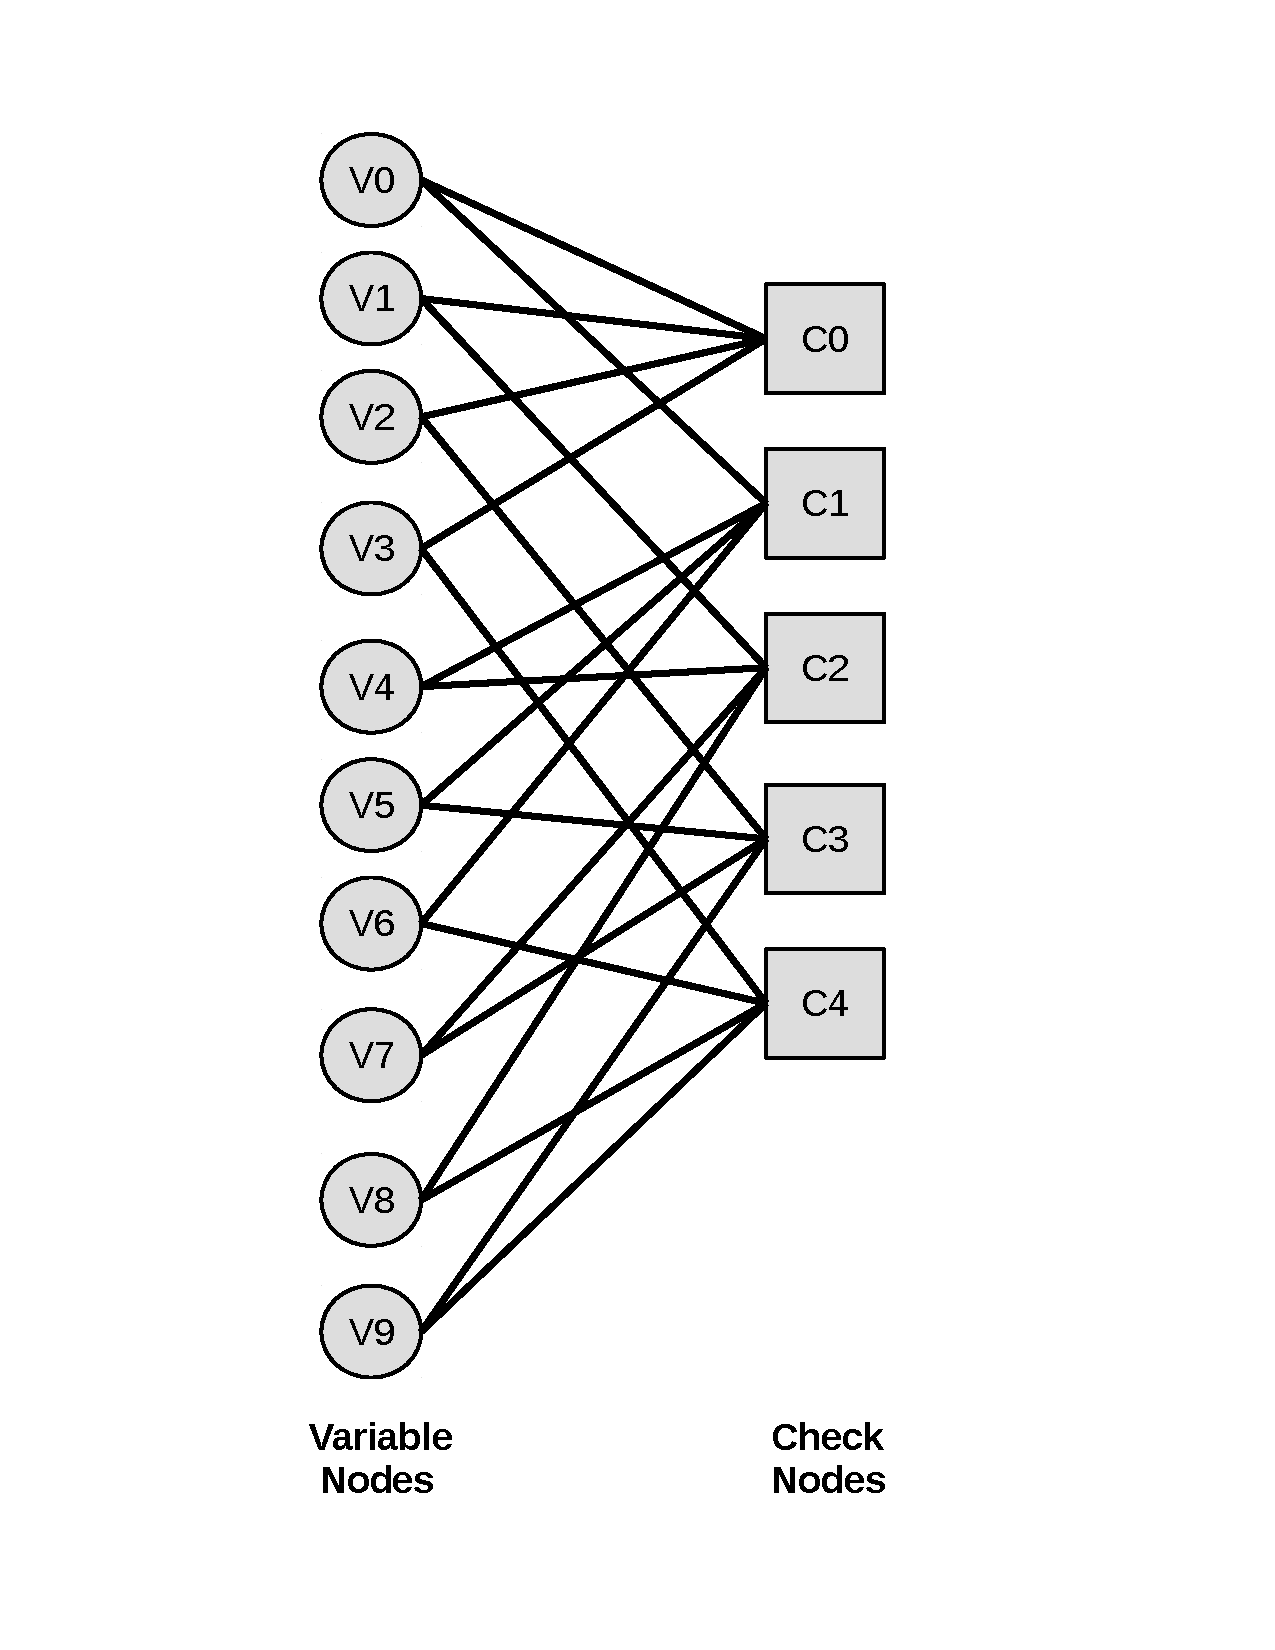
\includegraphics[scale=0.35]{tanner.pdf}
\caption[width=.3\textwidth]{An example of Tanner graph}\label{fig::tanner}
\end{centering}
\end{figure}

%Decoding
The general decoding algorithm of LDPC codes is based on the standard two-phase message passing (TPMP) principle described in \cite{art_massively}. This algorithm works in two phases. In the first phase, all the variable nodes send messages to their neighboring parity check nodes, and in the second phase the parity check nodes send messages to their neighboring variable nodes. Due to transcendental operations and relying of message passing algorithm to the estimation of noise standard deviation, in practice Min-Sum (MS) variants are prefered by designers \cite{art_neon}. This algorithm is provided in Algorithm 1.

\begin{algorithm}
\renewcommand\thealgorithm{}
\caption{\textbf{1} Min-Sum algorithm}\label{algorithm1}
\begin{algorithmic}[1]
\STATE \textbf{Loop 1:} Initialization
\FORALL{$m \in C, n \in V$}
%\IF{$H_{mn}==1$}
\STATE
$Lq_{nm}=0$%LP_n=\dfrac{2y_n}{\sigma^2}.$
%\ENDIF
\ENDFOR
\FORALL{$t=1 \rightarrow (iter\_max)$}
\STATE \textbf{Loop 2:} LLR of message $CN_m$ to $VN_n$
\FORALL{$m \in C, n \in V$}
\STATE $\alpha_{nm} \triangleq sign(Lq_{nm}),$
\STATE $\beta_{nm} \triangleq \abs{Lq_{nm}},$
\STATE $Lr_{mn} = \prod\limits_{n' \in N(m)\backslash n} \alpha_{n'm} \min\limits_{n' \in N(m)\backslash n} \beta_{n'm}.$
\ENDFOR
\STATE \textbf{Loop 3:} LLR of message $VN_n$ to $CN_m$
\FORALL{$m \in C, n \in V$}
\STATE $Lq_{nm} = LP_n + \sum\limits_{m' \in M(n)\backslash m} Lr_{m'n}.$
\ENDFOR  
\ENDFOR % End of Iter
\STATE \textbf{Loop 4:} Hard decision from soft-values
\FORALL{$n \in V$}
\STATE $LQ_{n} = LP_n + \sum\limits_{m' \in M(n)} Lr_{m'n},$
\STATE $\forall n, \hat{c}=[LQ_n]>0.$
\ENDFOR
\end{algorithmic}
\addtocounter{algorithm}{-1}
\end{algorithm}

One major drawback of Algorithm 1 is that, loops 2 and 3 are updated by separate processing and passed to each other iteratively. It means that update loop of the variable nodes, will not start until all check nodes are updated. This characteristic affects the efficiency of parallel implementation of such algorithm. 

Due to poor parallel mapping of Min-Sum algorithm, more efficient schedules, such as horizontal layered-based decoding algorithm, are proposed which allow updated imformation to be utilized more quickly in the algorithm, thus, speeding up decoding\cite{art_layered0, art_layered1}. In fact, the H-matrix can be viewed as a layered graph that is decoded sequentially. The work in \cite{art_gpu_0} has applied a form of layered belief propagation to irregular LDPC codes to reach 2x faster convergence for a given error rate. By using this method they have reduced memory bits usage by 45-50\%. The layered decoding (Algorithm 2), which is used in the proposed algorithm here, can be summarized as follow:
\begin{enumerate}
\item[$\bullet$] (1) All values for the check node computations are computed using variable node messages linked to them.
\item[$\bullet$] (2) Once, a check node is calculated, the corresponding variable nodes are updated immediately after receiving messages.
\item[$\bullet$] (3) This process is repeated to the maximum number of iterations.
\end{enumerate}

\begin{algorithm}
\renewcommand\thealgorithm{}
\caption{\textbf{2} Horizontal Layered Min-Sum algorithm}\label{algorithm2}
\begin{algorithmic}[1]
\STATE \textbf{Loop 1:} Initialization
\FORALL{$m \in C, n \in N(m)$}
\STATE
$Lr_{mn}^{(0)}=0$%LP_n=\dfrac{2y_n}{\sigma^2}.$
%\ENDIF
\ENDFOR
\FORALL{$t=1 \rightarrow (iter\_max)$}
\STATE \textbf{Loop 2:} For each check node
\FORALL{$m \in C$}
\FORALL{$n \in N(m)$}
\STATE$Lr_{nm}^{(t)}=E_n - Lr_{nm}^{(t-1)}$
\ENDFOR
\FORALL{$n \in N(m)$}
\STATE $\alpha_{nm} \triangleq sign(Lr_{nm}^{(t)}),$
\STATE $\beta_{nm} \triangleq \abs{Lr_{nm}^{(t)}},$
\STATE $Lr_{mn}^{(t)} = \prod\limits_{n' \in N(m)\backslash n} \alpha_{n'm} \min\limits_{n' \in N(m)\backslash n} \beta_{n'm}.$
\ENDFOR
\FORALL{$n \in N(m)$}
\STATE$E_n = Lr_{nm}^{(t)}+Lr_{mn}^{(t)}$
\ENDFOR
\ENDFOR
\STATE \textbf{Loop 3:} Hard decision
\FORALL{$n \in V$}
\STATE $\forall n, \hat{c}=[E_n]>0$
\ENDFOR
\ENDFOR % End of Iter
\end{algorithmic}
\addtocounter{algorithm}{-1}
\end{algorithm}
This project implements the layered decoding of LDPC codes on the GPU device of a mobile processor with high throughput and low latency performance. By using GPU device as the processing unit, significantly less resources of the ARM processor is used for decoding compared to similar work in \cite{art_neon}. Thus, there will be processing power left for other applications that need to be supported by the ARM processor. On the other hand, since the GPU and ARM of a mobile device are sitting on a same die, the latency issues in \cite{art_gpu_0} are improved.
%Although layered algorithm is composed of a single loop kernel composed to two sequential kernels in standard algorithms, it has an irregular memory access as a major limitation. To solve this irregular memory access, a data interleaving/deinterleaving process is used before and after the decoding process in \cite{art_gpu_0, art_neon}, which is used in the proposing algorithm too. 
%In \cite{art_gpu_0}, the GPU decoder achieves high throughputs but its latency that goes beyond seconds makes it suitable for simulation purposes only. On the other hand, the ARM decoder proposed in \cite{art_neon} uses all computing resources (4 existing cores) for LDPC decoding and does not take advantage of GPU processing on mobile devices. 
\section{Algorithm Mapping}\label{sec3}

An efficient implementation of the layered decoding algorithm is a challenging task. The drawbacks of this algorithm as in terms of programming are:
\begin{enumerate}
\item The number of computations with respect to the number of memory access is low.
\item The data reuse between consecutive computations is low.
\item It requires a large set of irregular memory access due to the sparse nature of the H-matrix \cite{art_ldpc_cpu1}.
\end{enumerate}
Considering these, a software-based decoder should take advantage of different parallelism levels offered by the target architecture to achieve high throughput efficiency. In this section, we detail the different parallelism levels, target architecture and the structure of proposed algorithm.

\subsection{Parallelism Levels in the Proposed Algorithm}
To achieve high throughput performance, a software based LDPC decoder has to exploit computational parallelism for taking advantage of multi-core architectures. Different parallelism levels are present in a layered decoding algorithm, which include:
\begin{itemize}
  \item[$\bullet$ ] First parallelism level is located inside the check node computations (Algorithm 2, loops located at line 8, 11 and 16). It is possible to execute such computations in parallel. However, this atomic parallelism level is hard to exploit due to the low complexity of computations.
\item[$\bullet$ ] Second parallelism level is located at the check node level (Algorithm 2, line 7). Two check node computations can be done in parallel if there is no data dependency. Since, this is rarely true, this level is hard to exploit and inefficient.
\item[$\bullet$ ] Third parallelism level is located at the frame level (Complete execution of Algorithm 2). The same computation sequence is executed over consecutive frames. This approach provides an efficient parallel processing algorithm. 
\end{itemize}
Hence, here, we use the SIMD programming model to decode F frames in parallel. In subsection \ref{subsec_proposed} the parallel decoding of F frames is referred to kernel 2 for sake of simplicity.
%In the next subsections, first the target architecture's features are presented. Then the structure of the proposed algorithm is detailed.

\subsection{Target Architecture} \label{target_architecture}
In this study, we focus on mobile embedded devices equipped with ARM and GPU processors. One example is Jetson K1 SoCs which consists of a 4-core Cortex-A15 and an NVIDIA GK20a GPU processor.

An ARM Cortex-A15 processor is composed of multiple integer and floating point pipeline stages and is capable of running multiple concurrent threads. As in terms of GPU features, concurrent kernel execution capability of this device is most used in the proposed mapping. To achieve high throughput performance on such a low-power embedded processors, SIMD and SIMT programming models are exploited in the proposed LDPC decoder. Although, the proposed structure is applicable to other heterogeneous structures too, and is not limited to embedded devices.

\subsection{Data Interleaving/Deinterleaving}
Recal that the implementation of the parallel frame processing is subject to massive irregular memory access due to the structure of H-matrix. As a matter of fact, to process the same $VN_i$ element of the F frames at the same time, non-contiguous memory access would affect performance. To solve this issue, a data interleaving process has to be performed before and after the decoding stage to ensure that each set of F frames are reordered to achieve an aligned memory data structure. This reordering is shown in Fig.\ref{fig_intreleave} \cite{art_ldpc_cpu1}. In the proposed structure, interleaving and deinterleaving of frames are called {kernel 1} and {kernel 3}.

\begin{figure}[h]
\begin{centering}
\scalebox{0.34}{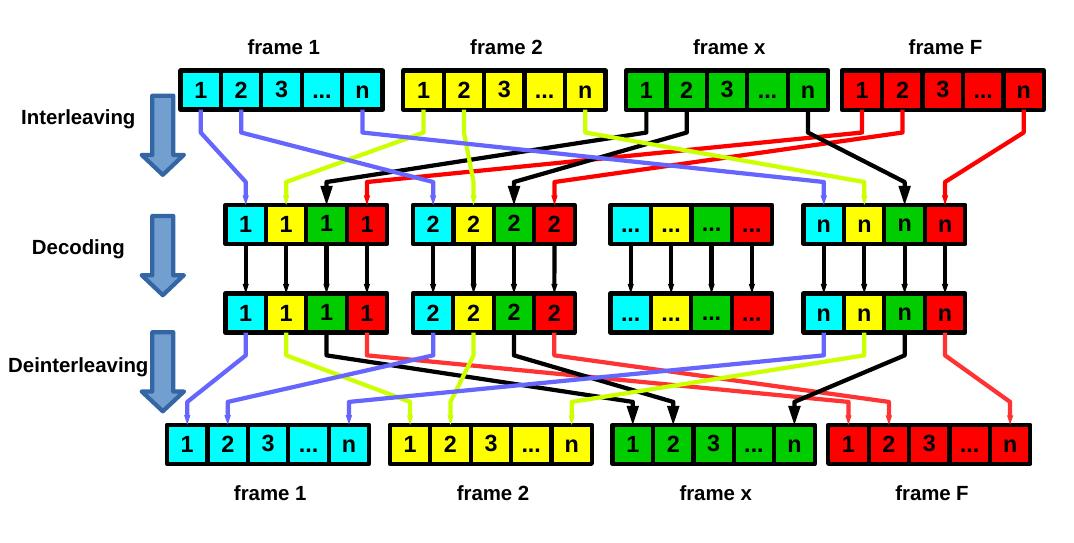
\includegraphics{inter1.jpg}}
\caption[width=.3\textwidth]{Data interleaving/deinterleaving process\cite{art_ldpc_cpu1}}
\label{fig_intreleave}
\end{centering}
\end{figure}

\subsection{Multi Stream Parallelism}\label{subsec_proposed}

The SIMT programming model is used to decode W sets of F frames concurrently, with W denoting the number of concurrent streams on the GPU device. This multi-core programming is specified by the CUDA API. Each GPU stream is controlled by a \textit{pthread} called \textit{worker} on the host machine (which is an ARM in this case). Each \textit{worker} is responsible for its own sets of frames. By using stream based processing, the system can decode W$\times$F frames at the same time. The whole LDPC decoder system model is shown in Fig.\ref{fig_total}.

\begin{figure}[h]
\begin{centering}
\scalebox{0.35}{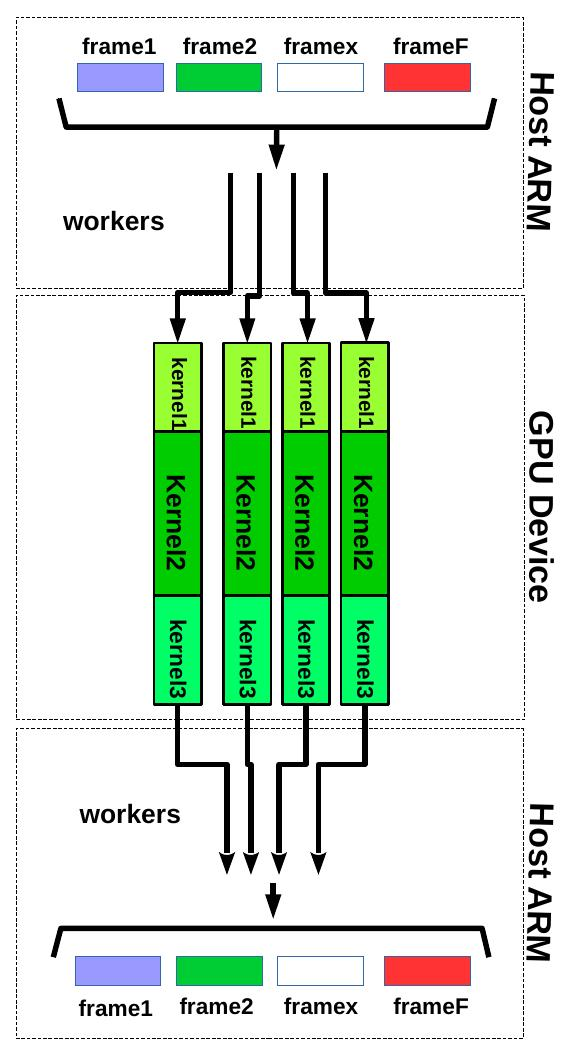
\includegraphics{total_new.jpg}}
\caption[width=.3\textwidth]{LDCP Decoder Data Flow}
\label{fig_total}
\end{centering}
\end{figure}

\section{Experimental Results} \label{sec4}

The experiments were carried out by decoding LDPC codes using NVIDIA Tegra K1 SoCs and various other structures to show scalability. The programs were compiled via GCC-4.8 and CUDA 6.5. The TK1 is composed of 4 cortex-A15 ARM processors and one NVIDIA Kepler "GK20a" GPU with 192 SM3.2 CUDA cores. The host platform uses a GNU/Linux kernel 3.10.40.

\begin{figure}[h]
\begin{centering}
\scalebox{0.15}{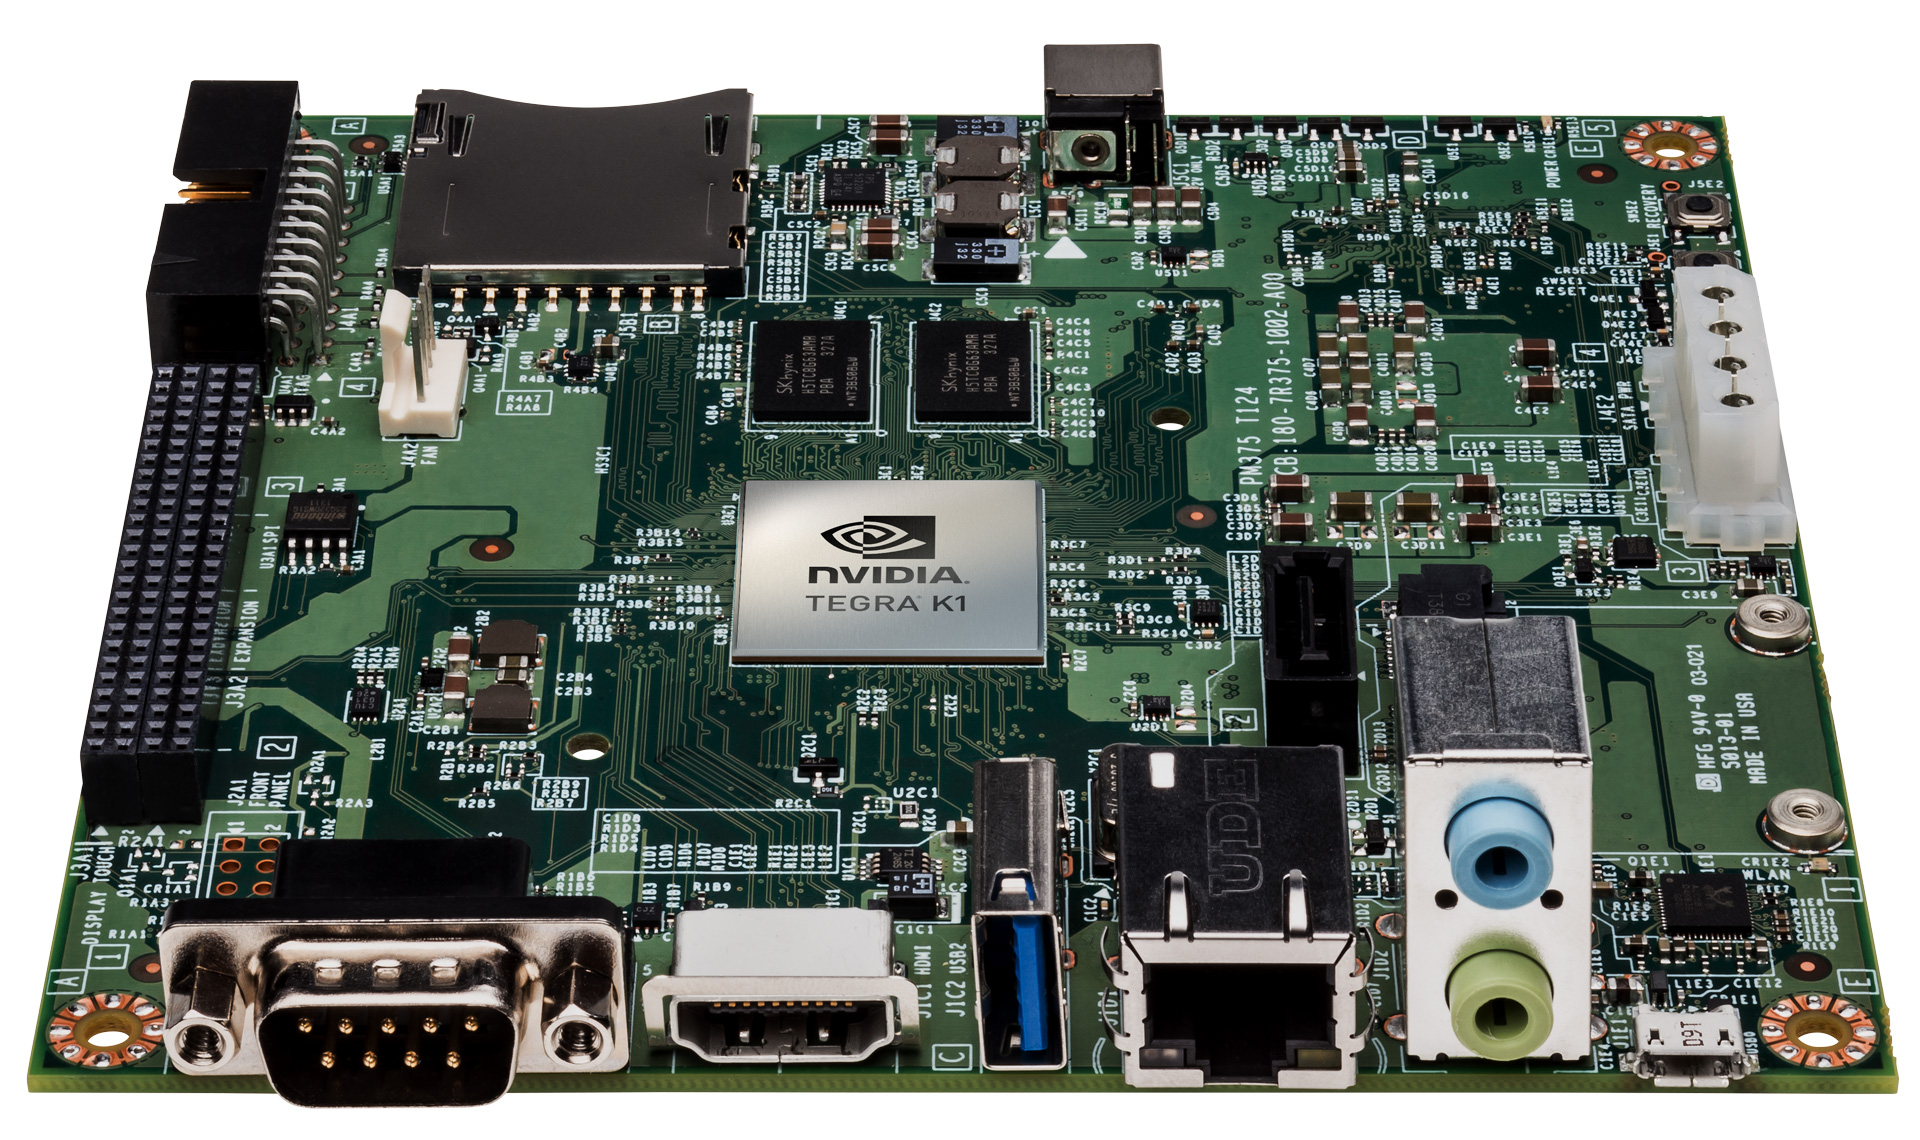
\includegraphics{Jetson_TK1.jpg}}
\caption[width=.3\textwidth]{Tegra-TK1 Development Board}
\label{tegra}
\end{centering}
\end{figure}

\subsection{Performance Evaluation of Proposed Algorithm} 
First set of experiments was performed to achieve air throughput using different codes. The codes have different frame lengths: 576 to 9972. The air throughputs are provided in Fig.\ref{fig::air} when \{1,3\} threads are used to handle \{1,3\} GPU streams. Measurements are performed for LDPC decoders that execute 10 layered-base decoding iterations.

Performance of one stream (or one thread) achieves 25 Mbps, while with 3 streams it can be as high as 35 Mbps. For a (4000,2000) LDPC code and one thread, data transfer takes about 2$\times$2.4 ms, interleaving steps need about 2$\times$5 ms and decoding takes about 150 ms. For the same code with 3 threads, data transfer takes about 2$\times$2.4 ms, interleaving steps need about 2$\times$5 ms and decoding takes about 150 ms. So by introducing more streams to GPU device, its performance does not degrade. In comparison the latency, i.e. the time for data transfer between the host and GPU device in \cite{art_gpu_0} is about 20 ms, which has been reduced here to 4.8 ms because of the architecture of embedded mobile device. On the other hand, with introducing 3 streams to GPU, its processing capacity is used more effectively which results to about 30\% throughput improvement in most of our experiments.

\begin{figure}[h]
\begin{centering}
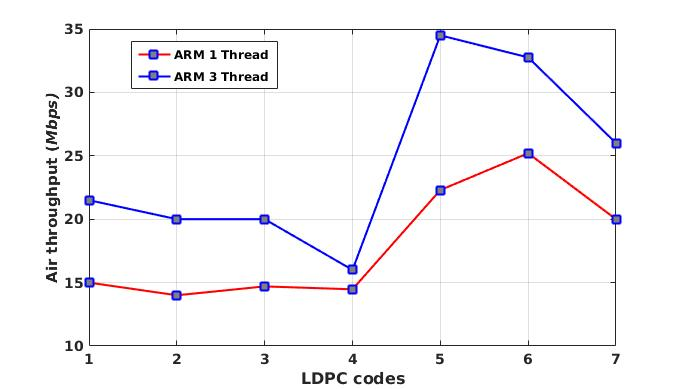
\includegraphics[scale=0.43]{air.jpg}
\caption[width=.5\textwidth]{Measured throughputs for 10 layered decoding iterations (1-7 LDPC codes: $576 \times 288, 1024 \times 512, 1200 \times 600, 1944 \times 722, 4000 \times 2000, 8000 \times 4000, 9972 \times 4086$)}\label{fig::air}
\end{centering}
\end{figure}

\subsection{Performance Comparison with Related Works}
To demonstrate the efficiency of the proposed ARM decoder, its throughput was compared to the ARM related work in \cite{art_neon}. In \cite{art_neon}, ARM SIMD units are used to perform vector data processing in parallel frame decoding. In the experiment, the throughput of the proposed decoder is compared to that of \cite{art_neon} while using 1 thread for the work in \cite{art_neon} and 3 threads in the proposed algorithm. This selection is motivated by the fact that the 1 thread from \cite{art_neon} uses a 100\% of a core while the 3 threads for the proposed algorithm only uses 8\% of each core resulting in an overall utilization of 24\%. 10-iteration decoding performed on Tegra-K1 board gives us the results as shown in Table \ref{table_compare_arm}. The work in \cite{art_neon} can achieve much higher throughputs by using more threads on the ARM processor, but by introducing each thread, the whole capacity of one more ARM core is used for decoding. In Table \ref{table_compare_arm}, it is shown that the proposed algorithm can achieve the similar throughput to that of \cite{art_neon} when using 24\% of ARM processing power and using its GPU device. Although, by using more powerful GPU device, the algorithm can achieve much higher throughputs which has been shown in next subsection. This shows that the proposed algorithm is scalable across platforms.
\begin{table}[H]
\centering
\caption{Throughput (Mbps) Comparison With Related Work} \label{table_compare_arm}
\resizebox{\columnwidth}{!}            & \textbf{34.5}                 & \textbf{\textit{24\%}}                 \\ \midrule
\textbf{(8000,4000)} & \textbf{34}              & \textbf{100\%}            & \textbf{33}                   & \textbf{\textit{24\%}}                \\ \bottomrule
\end{tabular}%
}
\end{table}

\subsection{Performance Comparison on Different GPU Devices}

GPU devices have different characteristics: amount of stream multiprocessors, CUDA cores, working frequencies, etc. A GPU based algorithm should have the scalability to use all the processing capability of a GPU device. In Table \ref{table:gpus}, the proposed algorithm has been executed on multiple GPU devices. GT540M and K620, are considered as mid-range and GTX680 and TeslaK20 are considered as high power GPU devices. The performance in Table \ref{table:gpus} shows that the proposed algorithm can achieve up to 230 Mbps performance across devices. In these set of experiments, an x86 CPU processor is the host.

\begin{table}[H]
\centering
\caption{Throughput (\textit{Mbps}) of algorithm on different GPUs}\label{table:gpus}
\begin{tabular}{@{}cc|c|cc@{}}
\toprule
\textbf{code}                        & \textbf{target}                    & \textbf{iter} & \textit{Mbps} (1-thread) & \textit{Mbps} (3-thread)  \\ \midrule
\multirow{8}{*}{\textbf{(576,288)}}  & \multirow{2}{*}{\textbf{GT540M}}   & \textbf{10}   & \textbf{23}  & \textbf{33}   \\ \cmidrule(l){3-5} 
                                     &                                    & \textbf{5}    & \textbf{44}  & \textbf{61}   \\ \cmidrule(l){2-5} 
                                     & \multirow{2}{*}{\textbf{K620}}     & \textbf{10}   & \textbf{23}  & \textbf{30}   \\ \cmidrule(l){3-5} 
                                     &                                    & \textbf{5}    & \textbf{45}  & \textbf{61}   \\ \cmidrule(l){2-5} 
                                     & \multirow{2}{*}{\textbf{GTX680}}   & \textbf{10}   & \textbf{94}  & \textbf{127}  \\ \cmidrule(l){3-5} 
                                     &                                    & \textbf{5}    & \textbf{163} & \textbf{217}  \\ \cmidrule(l){2-5} 
                                     & \multirow{2}{*}{\textbf{TeslaK20}} & \textbf{10}   & \textbf{66}  & \textbf{90}   \\ \cmidrule(l){3-5} 
                                     &                                    & \textbf{5}    & \textbf{123} & \textbf{165}  \\ \midrule
\multirow{8}{*}{\textbf{(2304,1152)}}& \multirow{2}{*}{\textbf{GT540M}}   & \textbf{10}   & \textbf{25}  & \textbf{37}   \\ \cmidrule(l){3-5} 
                                     &                                    & \textbf{5}    & \textbf{47}  & \textbf{63}   \\ \cmidrule(l){2-5} 
                                     & \multirow{2}{*}{\textbf{K620}}     & \textbf{10}   & \textbf{23}  & \textbf{31.5} \\ \cmidrule(l){3-5}
                                     &                                    & \textbf{5}    & \textbf{47}  & \textbf{63}    \\ \cmidrule(l){2-5}
                                     & \multirow{2}{*}{\textbf{GTX680}}   & \textbf{10}   & \textbf{94}  & \textbf{132}  \\ \cmidrule(l){3-5}
                                     &                                    & \textbf{5}    & \textbf{170} & \textbf{226}   \\ \cmidrule(l){2-5}
                                     & \multirow{2}{*}{\textbf{TeslaK20}} & \textbf{10}   & \textbf{66}  & \textbf{94}   \\ \cmidrule(l){3-5}
                                     &                                    & \textbf{5}    & \textbf{127} & \textbf{170}  \\ \midrule
\multirow{8}{*}{\textbf{(4000,2000)}}& \multirow{2}{*}{\textbf{GT540M}}   & \textbf{10}   & \textbf{27}  & \textbf{34}   \\ \cmidrule(l){3-5} 
                                     &                                    & \textbf{5}    & \textbf{27}  & \textbf{37}   \\ \cmidrule(l){2-5} 
                                     & \multirow{2}{*}{\textbf{K620}}     & \textbf{10}   & \textbf{24}  & \textbf{32}   \\ \cmidrule(l){3-5}
                                     &                                    & \textbf{5}    & \textbf{44}   & \textbf{60}   \\ \cmidrule(l){2-5}
                                     & \multirow{2}{*}{\textbf{GTX680}}   & \textbf{10}   & \textbf{98}  & \textbf{131}  \\ \cmidrule(l){3-5}
                                     &                                    & \textbf{5}    & \textbf{164}  & \textbf{230}  \\ \cmidrule(l){2-5}
                                     & \multirow{2}{*}{\textbf{TeslaK20}} & \textbf{10}   & \textbf{73}  & \textbf{98}   \\ \cmidrule(l){3-5}
                                     &                                    & \textbf{5}    & \textbf{139} & \textbf{196}  \\ \bottomrule
\end{tabular}
\end{table}

\section{Conclusion}
An stream-based approach for GPU-based LDPC decoding on embedded devices was introduced in this paper. This algorithm is based on running multiple concurrent kernels on GPU devices to utilize their processing capacity and freeing up resources on the ARM processor of mobile devices. Our results show that, this approach helps to achieve desirable throughputs on embedded mobile devices. Experimental results demonstrate that proposed algorithm is scalable and can achieve high throughputs on multiple GPU devices. Moreover, the proposed algorithm structure provides a trade off for the operating system to choose between performance and resource management by selecting various values for the number of streams that are used for decoding.

\newpage

\bibliographystyle{IEEEtran}
\bibliography{IEEEabrv,finalProject_bibliography}



\end{document}


